\documentclass{article}
% Chinese
% \documentclass[UTF8, nofonts, mathptmx, 12pt, onecolumn]{article}
% \usepackage{xeCJK}
% \setCJKmainfont{SimSun}
\usepackage{amsmath}
\usepackage{amsfonts}
\usepackage{amssymb}
\usepackage{wasysym}
% \usepackage{ctex}
\usepackage{graphicx}
\usepackage{float}
\usepackage{geometry}
\geometry{a4paper,scale=0.8}
\usepackage{caption}
\usepackage{subcaption}
% \newcommand{\oiint}{\mathop{{\int\!\!\!\!\!\int}\mkern-21mu \bigcirc} {}}
\newcommand*{\dif}{\mathop{}\!\mathrm{d}}
\newcommand*{\md}{\mathop{}\!\mathrm{d}}
\newcommand*{\me}{\mathrm{e}}

% \usepackage{parskip}
% \setlength{\parindent}{0cm}

\usepackage{bm}
\let\Oldmathbf\mathbf
\renewcommand{\mathbf}[1]{\boldsymbol{\Oldmathbf{#1}}}
\let\eqnarray\align

\author{Xiping Hu}
\usepackage{authblk}
\author{Xiping Hu}
\affil{http://thehxp.tech/}
\title{Homework for Chapter 2}

\begin{document}
\maketitle

\begin{figure}[H]
  \centering
  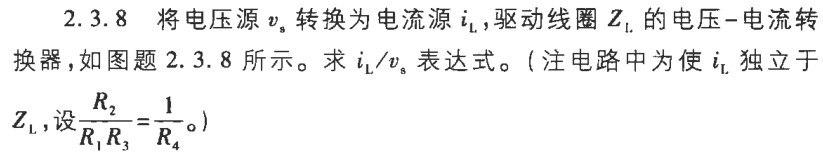
\includegraphics[width=0.9\linewidth]{figures/Problem1-0}
  \label{fig:}
\end{figure}

\begin{figure}[H]
  \centering
  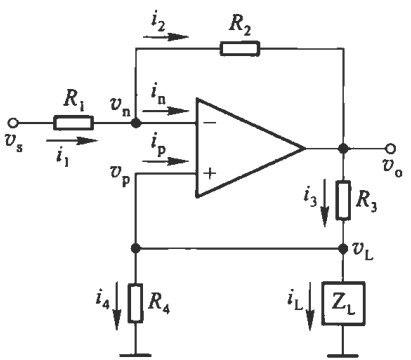
\includegraphics[width=0.4\linewidth]{figures/Problem1-1}
  \label{fig:}
\end{figure}

\paragraph{Solution}

Since we have $v_n = v_p = v_L = i_L Z_L$ and $i_n = i_p = 0$

\begin{equation*}
  \begin{aligned}
    i_1 &= i_2 \\
    i_3 &= i_4 + i_L
  \end{aligned}
\end{equation*}

Furthermore,

\begin{equation*}
  \begin{aligned}
  \dfrac{v_s - v_n}{R_1} &= \dfrac{v_n - v_o}{R_2} \\
  \dfrac{v_o - v_L}{R_3} &= \dfrac{v_L}{R_4} + \dfrac{v_L}{Z_L}   
  \end{aligned}
\end{equation*}

Then we have

\begin{equation*}
  \begin{aligned}
    \dfrac{v_s - i_L Z_L}{R_1} &= \dfrac{i_L Z_L - v_o}{R_2} \\
    \dfrac{v_o - i_L Z_L}{R_3} &= \dfrac{i_L Z_L}{R_4} + \dfrac{i_L Z_L}{Z_L}  
  \end{aligned}
\end{equation*}

So that

\begin{equation*}
  \begin{aligned}
    v_s &= \left( \dfrac{i_L Z_L - v_o}{R_2} \right) R_1 + i_L Z_L \\
    v_o &= i_L Z_L + \left( \dfrac{i_L Z_L}{R_4} + \dfrac{i_L Z_L}{Z_L} \right) R_3 \\
    v_s &= \left( \dfrac{i_L Z_L - \left( i_L Z_L + \left( \dfrac{i_L Z_L}{R_4} + \dfrac{i_L Z_L}{Z_L} \right) R_3 \right)}{R_2} \right) R_1 + i_L Z_L \\
    &= \left( \dfrac{ - \left( \dfrac{i_L Z_L}{R_4} + \dfrac{i_L Z_L}{Z_L} \right) R_3 }{R_2} \right) R_1 + i_L Z_L \\
    &= \left( \dfrac{ - \left( \dfrac{i_L Z_L}{R_4} + i_L \right) R_3 R_1 }{R_2} \right) + i_L Z_L \\
    &= \left( - \left( \dfrac{i_L Z_L}{R_4} + i_L \right) R_4 \right) + i_L Z_L \\
    &= - i_L Z_L - i_L R_4 + i_L Z_L \\
    &= - i_L R_4 \\
  \end{aligned}
\end{equation*}

Finally,

\begin{equation*}
  \begin{aligned}
    \dfrac{v_s}{i_L} = - R_4 
  \end{aligned}
\end{equation*}

\end{document}